\documentclass[preprint,12pt,authoryear]{elsarticle}
\journal{Journal of Systems and Software}
\biboptions{authoryear,round}
\usepackage[T1]{fontenc}
\usepackage[utf8]{inputenc}
\usepackage{lmodern}
\usepackage{amsmath,amssymb,amsthm}
\usepackage{booktabs,longtable,array,tabularx}
\usepackage{graphicx}
\usepackage{float}
\usepackage{url}
\usepackage{xurl}
\usepackage{hyperref}
\usepackage{microtype}
\usepackage{enumitem}
\providecommand{\tightlist}{\setlength{\itemsep}{0pt}\setlength{\parskip}{0pt}}
\graphicspath{{./}}
\hypersetup{colorlinks=true,urlcolor=blue,citecolor=black,linkcolor=black,pdfauthor={Oleksandr Kuznetsov}}
\emergencystretch=3em

\begin{document}
\begin{frontmatter}
\title{When Can a Blockchain Monitor Make a Decision? Source-Audited Feature Readiness, Historical State, and Exact-Execution Evidence}
\author[aff1,aff2,aff3]{Oleksandr Kuznetsov\corref{cor1}}
\cortext[cor1]{Corresponding author. ORCID: 0000-0003-2331-6326.}
\ead{oleksandr.kuznetsov@uniecampus.it}
\address[aff1]{Department of Theoretical and Applied Sciences, eCampus University, Italy}
\address[aff2]{Department of Intelligent Software Systems and Technologies, School of Computer Science and Artificial Intelligence, V.~N. Karazin Kharkiv National University, Ukraine}
\address[aff3]{SMARTEST Research Center, eCampus University, Via Isimbardi 10, Novedrate (CO), 22060, Italy}
\begin{abstract}
Monitoring silence can reflect missing observations, undefined scores or suppressed notifications. Across four Ethereum incident families and five documented executions, a daily-reset token-outflow rank notifies none; retained history yields matches for Bacon and Rari. Across twenty-two census emitters, 130 of 277 nonempty days (46.93\%) fail a necessary twenty-transaction gate. Comparison-contract measurements distinguish traffic feasibility from feature computability. Seven low-volume replays cannot establish prevalence. During Nomad's attack-day burst, a daily cap suppresses seven of twelve protocol-listed count candidates. Schnoodle's count rule matches one execution amid 27 notifications on 134 transactions; a token bucket with unit burst capacity suppresses that match at the same five-alert cap. These selected traces support separate validation of observation, causal computability, triggering and dispatch, without establishing population accuracy or exploit-mechanism recognition.
\end{abstract}
\begin{keyword}
Blockchain monitoring \sep Runtime monitoring \sep Empirical software engineering \sep Feature readiness \sep Historical initialization \sep Reproducibility
\end{keyword}
\end{frontmatter}

\section{Introduction}\label{sec:intro}
An automated monitor can evaluate a rule only when the required observation and prior state exist at decision time. Runtime verification distinguishes an available trace, the property being monitored and the monitor's answer \citep{Leucker2009RV,Bauer2011RV}; streaming anomaly evaluations likewise depend on warm-up rules and event time \citep{Lavin2015NAB}. A detection-rate figure can conceal a monitor that was unable to compute its intended feature on much of the evaluated workload.

We study this problem in Ethereum decentralized finance (DeFi). A monitoring pipeline selects transactions through nominated contract emitters, extracts features from their complete event bundles, updates historical state, scores observations, groups candidates and allocates notifications. Each stage imposes a distinct requirement. A user-to-attacker transfer may bypass a selected contract even when that contract emits another event in the attack transaction. A core-outflow monitor is therefore narrower than a transaction-wide exploit monitor; its security interpretation must match the documented mechanism \citep{Zhou2023SoKDeFi,Wu2024DeFiRanger,Meng2026Houston}.

Our starting observation was a negative result: a fixed daily-reset token-outflow rank notified no independently admitted execution in Li.Fi or Revest, whereas a count comparator matched one Li.Fi execution. We then replayed the complete selected streams under alternate history retention and examined Bacon Protocol and Rari Fuse Pool~127. These later cases and their observation boundaries were nominated before their new score outputs, but after the Li.Fi/Revest results were known. They constitute retrospective follow-up, not a fully blinded validation cohort.

The study asks where the monitor's input or state contract fails and whether initialization, security-feature meaning and dispatch can be distinguished. We address four research questions:
\begin{description}
\item[RQ1 (feature readiness).] How often does the observed traffic provide enough strictly preceding positive same-token outflows to compute the rank, and does end-of-day traffic overstate readiness at the documented execution?
\item[RQ2 (initialization and dispatch).] With transactions and decision rules fixed, how do history retention and notification allocation affect eligible scores and exact known-execution notifications? How does the count comparator behave on the same view?
\item[RQ3 (construct validity).] Do gross token outflows at the nominated core correspond to the security-relevant mechanism of the documented exploit?
\item[RQ4 (extension scope).] How do traffic feasibility, feature computability and notifications vary across additional emitter streams and event-count feature definitions, and which conclusions remain conditional on their sampling rules?
\end{description}

The primary study comprises four incident families and five admitted successful executions; overlapping Rari component views are not independent incidents. The extensions comprise twelve comparison emitters, twenty-two source-census emitters in twenty-three windows, seven low-volume replay views and a separate Nomad attack-day burst. We keep these units separate. The rank formula, minimum-history arithmetic and budget policies are not new methods. The contribution is an independently checked measurement procedure and empirical attribution of divergent monitoring outcomes to observation boundaries, historical state, score domain and dispatch. Explicit inclusion rules, source tiers and estimands limit what can be inferred from these selected traces \citep{Kitchenham2004Evidence,Wohlin2012Experimentation}.

\section{Related work and differentiation}\label{sec:related}
\paragraph{Runtime monitors and feature preconditions} Runtime verification evaluates properties over finite system observations \citep{Leucker2009RV,Bauer2011RV}. We do not verify a temporal-logic property or claim formal completeness. We measure a practical prerequisite: whether the observation and strictly prior state required by a score exist at the event being evaluated. An undefined feature is distinct from a defined low score. NAB emphasizes event-time detection evaluation \citep{Lavin2015NAB}; our evaluation unit is an exact blockchain transaction within a nominated component boundary.

\paragraph{DeFi exploit detection and semantics} TXSPECTOR studies transaction dependencies, EtherClue provides investigation-oriented indicators, and DeFiRanger models higher-level financial operations \citep{Zhang2020TxSpector,Aquilina2021EtherClue,Wu2024DeFiRanger}. HOUSTON evaluates richer protocol anomalies across a substantially larger incident collection \citep{Meng2026Houston}. Their detection rates are not directly comparable with our fixed-core rank/count rules because observations, labels and units differ. ERC-20-shaped transfers at one address need not represent native-ETH borrowing, user allowance abuse or accounting invariants \citep{Vogelsteller2015ERC20,Revest2022Postmortem,Rari2022Postmortem}.

\paragraph{Event provenance and boundaries} XChainWatcher applies logic-driven cross-chain event monitoring, and BridgeGuard studies cross-chain attack transactions \citep{Augusto2025XChainWatcher,Wu2025BridgeGuard}. Our Ethereum component views are narrower. Li.Fi's diamond architecture also separates entrypoint logs, implementation facets and user token transfers \citep{Mudge2020ERC2535,BlockSec2022LiFi}; observing one emitter does not establish complete protocol observation.

\paragraph{Empirical security evaluation} Security-ML methodology warns against unrealistic populations and unverified labels \citep{Sommer2010ClosedWorld,Arp2022Dons}. Empirical software engineering requires explicit units and inclusion criteria \citep{Kitchenham2004Evidence,Wohlin2012Experimentation}; hidden data and state dependencies are recognized sources of technical debt \citep{Sculley2015Debt}. DeFiHackLabs supplies exploit candidate code, not complete historical execution inventories \citep{DeFiHackLabs2026}. Forta documents practical monitoring interfaces without establishing the performance of our rules \citep{FortaDocs}. Our narrower question is whether numerical readiness, exact notification and security interpretation change together when historical state is retained.

\section{Monitoring model and estimands}\label{sec:model}

\subsection{Observation boundary, chronology and input units}
For each incident family $c$, a predeclared component view $v$ specifies one or more Ethereum log-emitting addresses. A transaction is \emph{selected} when at least one successful observed log is emitted by a view address. The full log bundle of a selected transaction is used to derive token-flow features, including transfer events from other emitters; selection itself does not use an attack label, anomaly score or transfer amount. Selected transactions are ordered by block number and transaction index. The block timestamp is a logical historical event time, not an observed network delivery time.

A \emph{case family} is a documented exploit event, not a row in an experiment table. Its \emph{core view} is a monitored component, not a separate attack; the Rari fETH, fUSDC and Comptroller views belong to one family. A \emph{known execution} is a historically identified and separately reviewed transaction that executed the documented unauthorized behavior. The verified inventories used here are \texttt{KNOWN\_SUBSET\_ONLY}; neither the negative population nor all historical exploit transactions are completely adjudicated. Therefore an emitted alert on an unknown transaction is not a false positive and a reference denominator is not a full incident recall denominator.

The extracted ERC-20-shaped fields are gross integer quantities as represented in the event data; they do not independently establish token compliance or a native-asset state delta. For token $k$, $x_{i,k}>0$ denotes the gross external token outflow whose sender is in the nominated view and whose recipient is outside it, as defined by the frozen extractor. Inflows do not cancel outflows. Different tokens have independent histories and raw units cannot be added across tokens without an external unit conversion \citep{Vogelsteller2015ERC20}.

\subsection{Feature readiness and the rank rule}
Let $H_{i,k}^{(m)}$ be the up-to-128 most recent strictly preceding positive values for token $k$ available at selected transaction $i$ under history mode $m$. The reported rank is
\begin{equation}\label{eq:rank}
q_{i,k}^{(m)}=\frac{1+\sum_{h\in H_{i,k}^{(m)}}\mathbf{1}\{h\geq x_{i,k}\}}{|H_{i,k}^{(m)}|+1}.
\end{equation}
A positive token score is eligible if $|H_{i,k}^{(m)}|\geq 19$. The primary semantic rule triggers on a selected transaction when at least one eligible token score has $q_{i,k}^{(m)}\leq1/20$; the separately reported sensitivity uses $1/10$. This empirical rank is not a calibrated transaction false-alarm probability. At 19 preceding positive values, a new value must be a strict maximum of the token's preceding amounts for $q\leq1/20$ to hold.

At a daily reset, a token-day with $N_{k,d}$ positive selected transactions permits at most $\max(0,N_{k,d}-19)$ eligible \emph{token scores}; it may produce fewer eligible transactions when multiple tokens occur in the same transaction. The inequality is a validation precondition, not a detection theorem. For a source-only necessary bound, let $T_{v,d}$ denote all distinct selected transactions for view $v$ on day $d$; if $T_{v,d}<20$, no token can have an eligible daily-reset score that day. Crucially, for a specific reference transaction $i$, the relevant necessary bound is $T_{v,d}^{\mathrm{prior}}(i)\geq19$, the number of distinct view-selected transactions \emph{strictly before} $i$ on that day. End-of-day totals include post-attack traffic and are not an acceptable proxy for this condition.

\subsection{History-policy intervention}
Three modes are replayed over the \emph{same} retained 30-day historical window:
\begin{enumerate}
\item \textbf{Daily reset:} remove positive-token histories at each UTC midnight.
\item \textbf{Trailing seven days:} keep qualifying positive observations from earlier transactions in blockchain order whose timestamps lie in $[t_i-7\,\mathrm{days},t_i]$, capped at 128 per token. Earlier transactions in the same block may share $t_i$; the current and later transactions are excluded.
\item \textbf{Cumulative in the captured window:} retain positive observations from the beginning of the available 30-day window, also capped at 128 per token.
\end{enumerate}
All modes use the same positive-flow definition and start cold at the beginning of the captured window; they do not represent a monitor initialized from unrestricted earlier chain history. Daily reset was an operational source-partition choice, not a blockchain requirement. The historical alternatives were introduced after initial Li.Fi/Revest exposure.

\subsection{Grouping, count comparator and notification allocation}
A raw trigger becomes a grouped candidate when no previous grouped candidate exists that UTC day, or its time gap from the previous grouped candidate is \emph{at least} 300 seconds ($\Delta t\geq300$ s). A trigger strictly inside that interval is suppressed and does not advance the grouping anchor. The anchor is the previous grouped candidate, even if its notification was rejected by the budget; it is not the previous emitted alert. The count comparator triggers when at least ten core-emitter logs occur in $(t-60\,\mathrm{s},t]$, including the complete current transaction. It needs no token history and its rolling state resets daily.

For each day the notification allocator receives the grouped candidates and enforces an offered maximum $B\in\{1,5,20\}$, under greedy, paced-cumulative and token-bucket admission. No rejected candidate is queued. Budget-policy state resets daily for every feature-history mode. Offered capacity and realized notifications are reported separately: a nominal $B=5$ does not imply five messages. Comparisons in the main tables use the primary rank $1/20$, greedy admission and $B=5$, with all policy and threshold variants retained in machine-readable results.

Greedy admission sends each grouped candidate until the daily cap is reached. Paced cumulative admission permits at most $\min\{B,1+\lfloor B\tau/86400\rfloor\}$ messages by $\tau$ seconds after UTC midnight. The token bucket has capacity one, starts each day with one token, refills at $B/86400$ tokens per second and consumes one token per emitted candidate; the same hard daily cap $B$ also applies. Its offered daily maximum is therefore not an assurance of immediate capacity for clustered candidates.

\subsection{Outcomes and independent checks}
The operational record preserves source observation, core selection, feature eligibility, raw/grouped candidates and emitted alerts. In the A--D summary below, source observation and core selection form A, feature eligibility forms B, triggering forms C, and grouping/allocation form D. Label-free readiness is the number of selected transactions with at least one eligible score divided by the selected transaction count. Exact known-set coverage is the number of independently admitted execution transactions that have themselves emitted alerts divided by the number of such known executions within the selected scope. The latter is descriptive; missing labels preclude estimation of precision, false-positive rate or incident-wide recall.

\section{Primary study material and protocol}\label{sec:material}
\subsection{Four incident families and fixed component views}
Table~\ref{tab:cohort} defines the primary units. Li.Fi/Revest each contribute thirty days ending on the incident date: sixty case-days cover thirty-seven distinct UTC dates. Bacon's window is 4 February--5 March 2022, and Rari Pool~127's is 1--30 April 2022. Shared dates, tokens or Rari views do not create additional independent incidents.

\begin{table}[htbp]
\centering\footnotesize
\caption{Four incident families and fixed observation boundaries. Counts are case-specific; Rari component views overlap. All execution inventories are known subsets.}
\label{tab:cohort}
\begin{tabular}{p{1.8cm}p{3.35cm}c p{2.7cm}c}
\toprule
Incident & Observed components & Days & Selected TX & Known refs \\
\midrule
Li.Fi & Diamond entrypoint & 30 & 280 & 1 \\
Revest & Entrypoint and TokenVault & 30 & 194 & 2 \\
Bacon & Lending proxy & 30 & 256 & 1 \\
Rari Pool~127 & fETH; fUSDC; Comptroller (separate) & 30 & 132; 159; 133 (411 union) & 1 (shared) \\
\bottomrule
\end{tabular}
\end{table}

\subsection{Selection and protocol chronology}
An earlier thirteen-entry catalogue yielded three named-component nominations, six unresolved metadata/core nominations, and four development or non-realized dispositions. Li.Fi and Revest passed its historical reference and source gates. A later version-pinned DeFiHackLabs screen examined Bacon, Rari, Umbrella, Auctus and Saddle. Bacon and Rari Pool~127 passed; unresolved core or reference roles for the other three remain recorded, not labelled negative.

The seven-day and cumulative-history implementations were checked at commit \texttt{b20bde6} after initial Li.Fi/Revest exposure. The Bacon/Rari cohort, scoring and postscore-join protocol was fixed at \texttt{33536e9} before their accepted replay at \texttt{9a13e60}. Thus the algorithm preceded those scoring results, but case selection remained incident-informed. The artifact retains full commit hashes, timestamps and all dispositions.

Li.Fi's incident used existing user allowances through an unchecked external call \citep{LiFi2022Postmortem,BlockSec2022LiFi}; Revest involved reentrant FNFT collateral accounting \citep{Revest2022Postmortem,SlowMist2022Revest}. Bacon was reported as a lending-workflow reentrancy, with incomplete implementation verification limiting reconstruction of the internal path \citep{Bacon2022Postmortem,Certik2022Bacon}. Rari's team described native-ETH borrowing and \texttt{exitMarket()} reentrancy across multiple Fuse pools; we evaluate one original Pool~127 transaction \citep{Rari2022Postmortem,Beosin2022Rari}.

\subsection{Source tiers and independent replay}
Li.Fi/Revest observations originate in enumerated AWS Ethereum Parquet partitions with selected all-emitter transaction bundles. For Bacon/Rari, original address projections and transaction identities fix chronology and core-emitter counts; Blockscout supplies the complete indexed \texttt{topics}, \texttt{data} and successful-status records for those selected identities. Agreement in identities and counts does not authenticate Ethereum receipt roots \citep{AWS2026Dataset}. The original third-party Parquet bodies are not redistributed.

Bacon contains 256 selected transactions; Rari contains 411 distinct union-selected transactions across fETH (132), fUSDC (159) and Comptroller (133) views. Their known executions contain 18 and 65 all-emitter logs, respectively. For all ten distinct Bacon/Rari transactions in the primary notification-and-reference ledger, a further original-Parquet comparison confirmed exact event payload, address and order agreement with the normalized indexed data. This targeted check does not authenticate statuses or every selected transaction.

The primary configuration is rank $1/20$, greedy daily budget $B=5$ and 300-second grouping. Retention changes only the token-rank state. The original sealed comparisons were independently reproduced (948 method rows and 8,532 policy rows); alternate-history replay retains 108 semantic configurations for Li.Fi/Revest. A separate implementation reproduced all 252 Bacon/Rari method-policy cells with identical emitted transaction sequences. These configuration counts describe calculation checks, not independent attacks or training runs.

OpenAI ChatGPT and Codex assisted development of the acquisition, replay and verification scripts. Released replay and verification code contains no language-model inference and is checked through archived inputs and separately implemented calculations.

\section{Primary results}\label{sec:results}
\subsection{RQ1: feature readiness across the observed streams}
The original daily-reset streams contain 141 Li.Fi and 102 Revest selected transactions with positive external core outflow. At the required minimum 19 preceding positive values, no Li.Fi transaction is eligible and only 24 of Revest's 194 selected transactions are eligible. Li.Fi has 83 positive token-days, none containing the 20 qualifying transactions required to compute even a first eligible rank. Revest has 17 positive token-days, of which one reaches the threshold. Thus a failure to notify the known execution is not the only measurable symptom; most of the corresponding observation stream cannot enter the rank decision at all under this initialization.

Table~\ref{tab:eligibility} extends this check across all six fixed core views. Retaining history strictly before the scored transaction raises the proportion of defined scores, but the extent differs markedly by observed token stream. The Comptroller view in the retained Rari population yields no positive gross core outflow at all; longer history cannot repair this feature-definition mismatch.

\begin{table}[htbp]
\centering\small
\caption{Transactions with at least one eligible positive token score when at least 19 prior values are required. The fraction is conditional on the named core-selected transaction population; Rari views overlap.}
\label{tab:eligibility}
\begin{tabular}{lrrrr}
\toprule
View & Selected TX & Daily reset & Trailing 7 d & Captured 30 d \\
\midrule
Li.Fi core & 280 & 0 & 20 & 59 \\
Revest core & 194 & 24 & 64 & 71 \\
Bacon proxy & 256 & 0 & 0 & 15 \\
Rari fETH & 132 & 0 & 5 & 23 \\
Rari fUSDC & 159 & 1 & 36 & 75 \\
Rari Comptroller & 133 & 0 & 0 & 0 \\
\bottomrule
\end{tabular}
\end{table}


A simple sensitivity analysis of minimum strictly preceding history lengths 1, 5, 10, 19 and 39 is reported as a machine-readable table for each view and initialization policy. This is \emph{not} a retrospective optimization of a detector threshold: the corresponding score triggering and exact-execution comparisons retain the original history minimum of 19. The sensitivity exposes how much workload remains eligible under alternative preconditions rather than suggesting an improved detection rate.

\subsection{Attack-time readiness, not end-of-day volume}
The additional Bacon/Rari audit allowed us to distinguish the number of selected transactions by the end of the incident day from those that precede the known exploit. Table~\ref{tab:attacktime} separates whole-day volume from the information available before the execution. In fact, three of four component views record 20 or more selected transactions over the full incident day, but \emph{none} has 19 selected transactions strictly before the reference execution. The reference transaction itself is scored before its positive amount is appended to history.

\begin{table}[htbp]
\centering\footnotesize
\caption{Selected transactions on the documented attack day. The current execution is excluded from strictly preceding history. Four views belong to only two incident families.}
\label{tab:attacktime}
\begin{tabular}{lrrrrp{2.5cm}}
\toprule
View & Full day & Before & Ref. & After & Max earlier positive same-token values \\
\midrule
Bacon proxy & 23 & 2 & 1 & 20 & 0 \\
Rari fETH & 19 & 8 & 1 & 10 & 7 \\
Rari fUSDC & 48 & 17 & 1 & 30 & 11 \\
Rari Comptroller & 24 & 18 & 1 & 5 & 0 \\
\bottomrule
\end{tabular}
\end{table}

\begin{figure}[htbp]
\centering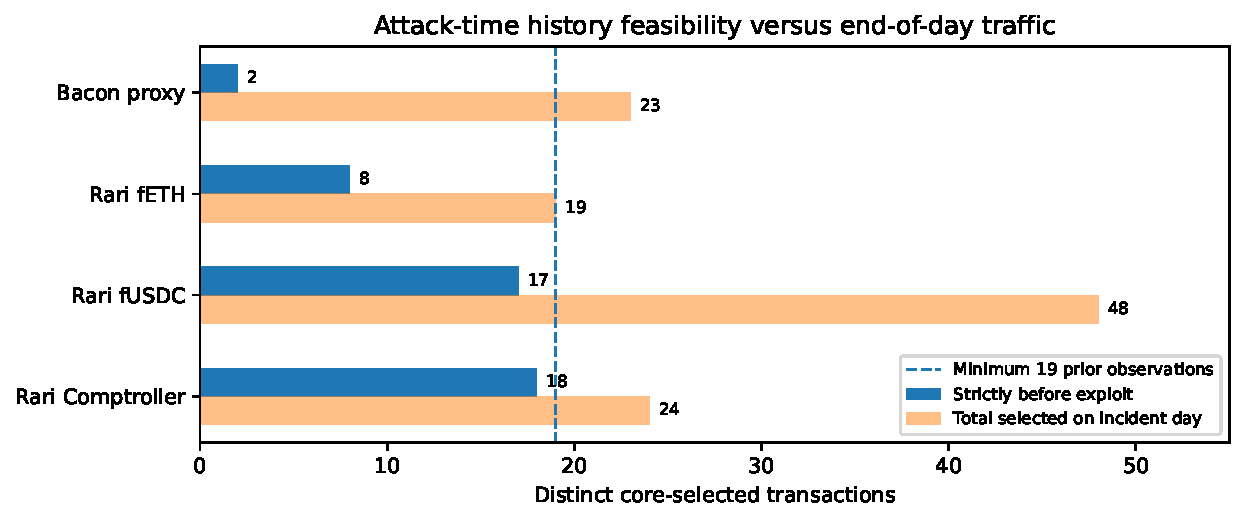
\includegraphics[width=\linewidth]{fig1_attack_time_selected.pdf}
\caption{Source-validated distinct transactions strictly before the documented execution (dark bar) versus the full day including the execution and subsequent traffic (light bar). The dashed line denotes the necessary 19 preceding selected transactions; the stricter feature-specific condition requires 19 earlier \emph{positive same-token outflows}.}
\label{fig:attacktime}
\end{figure}

None of these four views supplies 19 prior positive same-token outflows at the reference execution. Their daily-reset misses therefore have a measured eligibility explanation; full-day totals cannot replace strictly preceding history.

\subsection{RQ2: history initialization, count comparator and exact notifications}
Table~\ref{tab:outcomes} compares exact known-reference notifications with the total number of emitted messages under the primary greedy daily budget. An entry such as $1/3$ means that one known reference execution was notified in a three-alert stream; it is \emph{not} an estimate of precision. The count comparator is independent of rank-history mode and appears as its own reference column.

\begin{table}[htbp]
\centering\scriptsize
\caption{Primary outcomes as \emph{exact known-execution hits / all emitted notifications} (greedy, $B=5$, rank threshold $1/20$). No unknown notification is treated as a false positive. Three Rari views share one historical execution.}
\label{tab:outcomes}
\begin{tabular}{lrrrr}
\toprule
View & Semantic daily & Semantic 7 d & Semantic 30 d & Count daily \\
\midrule
Li.Fi core & 0/0 & 0/0 & 0/2 & \textbf{1/1} \\
Revest core & 0/0 & 0/2 & 0/1 & 0/2 \\
Bacon proxy & 0/0 & 0/0 & \textbf{1/1} & 0/1 \\
Rari fETH & 0/0 & \textbf{1/1} & \textbf{1/3} & 0/0 \\
Rari fUSDC & 0/0 & \textbf{1/2} & \textbf{1/7} & \textbf{1/2} \\
Rari Comptroller & 0/0 & 0/0 & 0/0 & \textbf{1/1} \\
\bottomrule
\end{tabular}
\end{table}

The original negative outcome persists for Li.Fi and Revest: greater historical readiness yields additional alerts but no exact known execution notification. Li.Fi's cumulative replay yields two unadjudicated notifications, on 1 and 3 March 2022, preceding the 20 March exploit. The Revest seven-day mode yields two unadjudicated notifications on 23 and 24 March, and cumulative history yields one on 24 March. These are not credited as early detections because no independently established relation to the attack has been shown.

By contrast, the new case results differ. Bacon's cumulative within-window history yields a reference-execution notification at 12:46:23 UTC on 5 March 2022: the USDC rank is $1/33$ after 32 strictly preceding positive core-outflow values. The trailing-seven-day history contains only five such values and cannot score that transaction. In Rari fETH, the known execution is notified under seven-day and cumulative histories with scores $1/24$ and $1/42$. In Rari fUSDC, independently recomputed seven-day scores are $1/27$ for USDC (26 previous observations) and $1/23$ for fUSDC (22 previous observations); the respective captured-window scores are $1/64$ (63 previous) and $1/34$ (33 previous). The two tokens are scored on one view of the same known Rari transaction, not independent incident hits. The Comptroller has no positive core-boundary token outflow, so no semantic trigger occurs, while the count comparator notifies the known execution. These are observation-view-dependent matches on one shared Rari execution, not multiple independent attacks.

Across all primary 1/20 cells in the new two-family replay, the offered budget never blocks an eligible grouped semantic candidate. Under the more permissive rank $1/10$, grouping and allocation can change realized loads; all retained policy/budget cells remain available in the result export. The main outcome is therefore driven principally by feature readiness, component observation and rank extremeness rather than budget exhaustion. Budget studies on the separate, previously exposed Euler and Beanstalk development workloads are not pooled into this external table; their event-time allocation findings answer a different question.

\subsection{Alert timing and reference status}
The primary semantic comparison produces a 19-row notification ledger retaining view, event time, token, rank, history policy, transaction hash and reference status (\ref{app:alerts}). Fourteen rows do not match the admitted execution inventory; they represent twelve distinct transactions. These remain unadjudicated, even when their timing precedes an exploit. Figure~\ref{fig:alerttime} reports event-time offsets, not live warning latency.

\begin{figure}[htbp]
\centering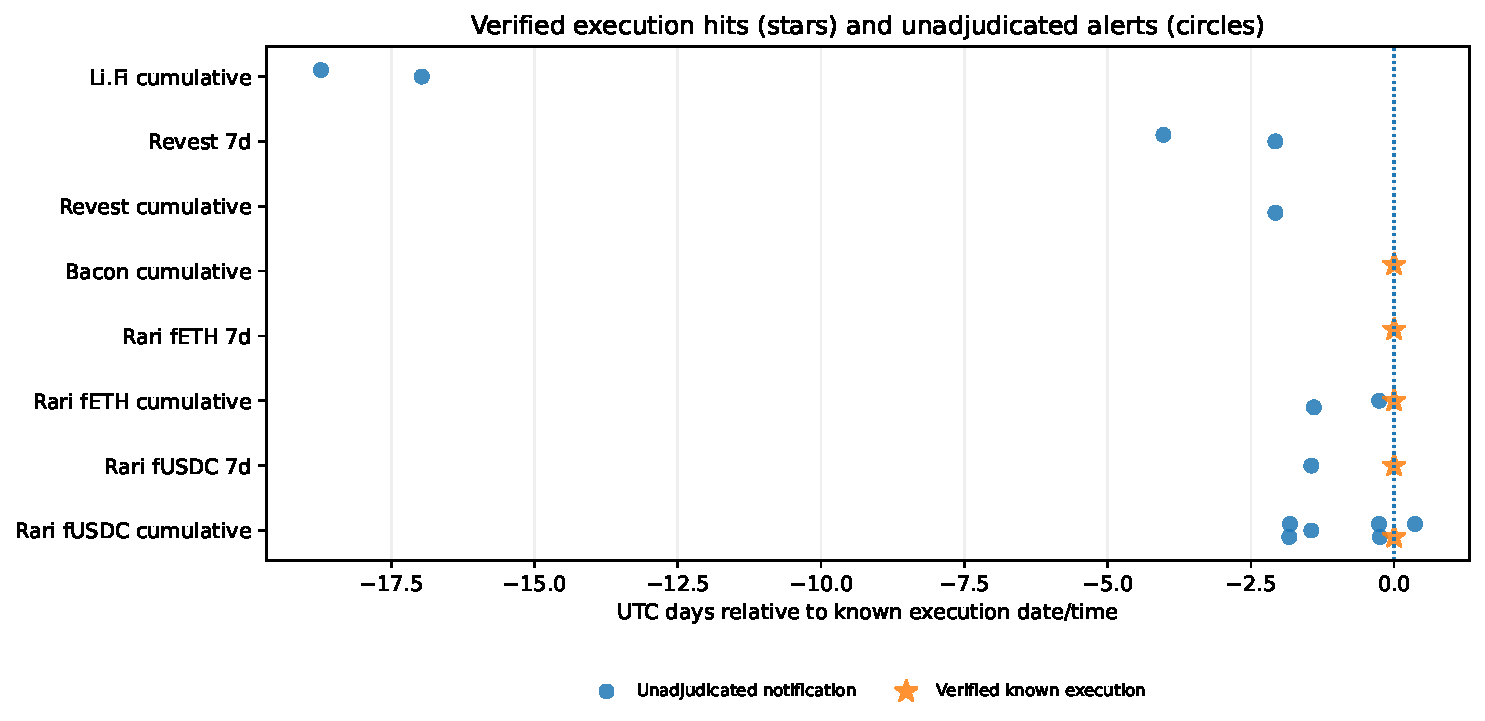
\includegraphics[width=\linewidth]{fig2_incident_relative_alerts.pdf}
\caption{Timing of primary semantic notifications relative to the documented execution time. Stars mark notifications on the exact admitted reference, and circles denote unadjudicated notifications. Rari rows share the same reference execution; Li.Fi and Revest reference times come from the independently admitted historical identities. A small deterministic vertical displacement separates overlapping plotted notifications without changing their time coordinates. The graph does not establish early warning or live notification latency.}
\label{fig:alerttime}
\end{figure}

\subsection{RQ3: feature--mechanism correspondence}
The original Li.Fi post-mortem and independent attack analysis describe an external-call/approval route: user funds could be transferred through allowances granted to the protocol \citep{LiFi2022Postmortem,BlockSec2022LiFi}. The reference transaction contains 40 ERC-20-shaped logs, of which only three touch the monitored diamond core; 92 logs were emitted across the transaction. The positive USDC/USDT core-boundary flows used by the rank rule are not the victim-to-attacker transfers themselves. With cumulative history, the Li.Fi USDC rank on the reference is $54/56$, not a high-outflow anomaly. This is a construct limitation independent of the original daily-history ineligibility.

Revest's admitted reference tokens have no strictly preceding positive outflows in the retained 30-day history, despite positive flows at the known executions; its documented exploit relates to reentrancy and FNFT accounting rather than an isolated magnitude tail \citep{Revest2022Postmortem,SlowMist2022Revest}. In Bacon, an exact rank notification appears under cumulative history, but a positive USDC transfer at the lending proxy is not by itself proof that the statistic recognizes the underlying reentrancy mechanism. In Rari, the fETH token outflow event and fUSDC ERC-20 transfer patterns are similarly not interchangeable with the principal native-ETH borrowing/state update exploit mechanism documented by the team \citep{Rari2022Postmortem}. Exact transaction coincidence is measurable and meaningful; precise exploit-mechanism recognition is a stronger claim that these syntactic features do not establish.

The source-tier, component-role and token/transaction distinctions thus matter to requirements engineering for a monitor. Before treating a rule as an exploit detector, a specification must state which class of adversarial state transition the feature is intended to represent, which contracts must be observed, and whether the feature is available strictly before the requested decision. This does not turn the studied rank statistic into a new attack-specific detector.

\section{Extension studies (RQ4)}\label{sec:extensions}
\subsection{Comparison-contract feature domains}
A separate convenience sample comprises twelve publicly documented lending, AMM and vault emitters over the same two thirty-day windows as Bacon/Rari: twenty-four contract--window pairs and 720 contract-days. Its registry and feature definitions were fixed before acquisition. These contracts have unknown attack status; they are not verified benign controls. Eleven emitters exceed nineteen selected transactions on every day in both windows (660 days); Curve AAVE fails that count gate throughout (60 days).

This extension uses \emph{core-emitter logs per selected transaction}, not positive ERC-20 outflows. The 714,951 event-count observations support three computability checks: rolling z-score and MAD on the nineteen most recent prior samples with positive dispersion, and EWMA with five prior samples. Table~\ref{tab:runtime} shows that abundant transactions do not guarantee a valid score domain. Daily-reset MAD is defined for only 1.93\% of observations, versus 38.50\% for z-score and 99.52\% for EWMA. These percentages are feature-domain measurements, not token-rank readiness or detection accuracy. Historical state is bounded by the captured window.

\begin{table}[htbp]
\centering\small
\caption{Actually computable event-count features in the 12-contract comparison census ($714{,}951$ transaction observations; 720 dependent contract-days). The cumulative mode begins without pre-window state. A defined score domain differs from an alarm or an attack label.}
\label{tab:runtime}
\begin{tabularx}{\linewidth}{@{}>{\raggedright\arraybackslash}X r r@{}}
\toprule
Feature definition & \shortstack{Daily reset\\ready (\%)} & \shortstack{Retained window\\ready (\%)}\\
\midrule
Rolling z-score (19; nonzero variance) & 275,250 (38.50) & 283,909 (39.71)\\
Rolling MAD (19; positive MAD) & 13,816 (1.93) & 14,857 (2.08)\\
EWMA (warm-up 5) & 711,525 (99.52) & 714,831 (99.98)\\
\bottomrule
\end{tabularx}
\end{table}

\subsection{Catalogue-complete source-traffic census}\label{sec:sourcecensus}
The completed frame includes every Ethereum-mainnet PoC file in the March--September 2022 directories of the immutable DeFiHackLabs snapshot \citep{DeFiHackLabs2026}, except the four primary-study files. The artifact's \texttt{CATALOGUE\_COVERAGE.json} accounts for all 67 Solidity files: 39 use other chains and 28 use Ethereum. Its 24 extension files map to 22 nominated component emitters and 23 distinct emitter/fork windows. Both Circle forks are retained; the two XST files share one emitter and fork and therefore one window. Sixteen windows were originally nominated before their traffic was measured; eight omitted files were added after review, with their component boundaries fixed before acquisition. Coverage is complete for this frozen catalogue and period; component choices remain investigator-interpreted, and unrealized PoCs and unresolved roles remain included.

For each distinct emitter/fork pair, a thirty-UTC-day window ends on the date of its PoC fork block. The anchor supplies a reproducible historical source context, often before the documented exploit; it is useful for studying potential pre-incident history. It is not an exact attack-time cut-off: the final UTC date includes transactions after the fork, and the exploit can lie outside the window. Attack-time readiness therefore requires a separate strict cut-off at the documented transaction. Beanstalk illustrates the distinction: its frozen source window ends on 16 April, whereas its exploit is on 17 April 2022.

Every original AWS daily log object and row group was projected onto emitter, block and transaction index; accepted byte ranges retained source identities and SHA-256 receipts. All 23 windows completed without imputing failed acquisitions as zero. The primary summary deduplicates emitter/UTC-date pairs: Circle's windows share 27 dates, leaving 663 distinct emitter-days and 51,452 emitter-specific selected-transaction observations. These are not globally distinct transactions. The secondary window-multiplicity summary has 690 days and 54,492 observations. This census measures selected-transaction count $T_{c,d}$ only: $T_{c,d}<20$ rules out a daily token rank, whereas $T_{c,d}\geq20$ does not establish positive same-token history.

Of 277 nonempty emitter-days, 130 (46.93\%) contain fewer than twenty selected transactions; 386 additional days are silent (Table~\ref{tab:newframe}). The original sixteen-window result remains 108/178 (60.67\%); the expanded frame changes this descriptive fraction. Creation dates are resolved for all 22 addresses from preserved indexed metadata. All 214 strictly predeployment dates are silent. Excluding them leaves 302/449 days (67.26\%) below twenty; also excluding the ten partially observed creation dates leaves 293/439 (66.74\%). These deployment-conditioned figures include deployed but silent days and differ from the nonempty-day estimand. Ronin and Beanstalk exceed nineteen transactions on every captured day; Schnoodle does not on any of its twenty-nine nonempty days.

\begin{table}[htbp]
\centering\small
\caption{Source audit across 22 nominated emitters. Each emitter/UTC-date pair is counted once, including the overlap of Circle's two windows. Silent dates include predeployment, inactive and unused-emitter dates; creation-conditioned sensitivity is reported separately.}
\label{tab:newframe}
\begin{tabularx}{\linewidth}{@{}>{\raggedright\arraybackslash}X r r@{}}
\toprule
Emitter-selected transactions in UTC day & \shortstack{Emitter-\\days} & \shortstack{Share of 663\\days}\\
\midrule
Exactly zero & 386 & 58.22\%\\
From 1 to 19 & 130 & 19.61\%\\
20 or more & 147 & 22.17\%\\
\midrule
All days & 663 & 100.00\%\\
\bottomrule
\end{tabularx}
\end{table}

Figure~\ref{fig:newframe} and \ref{app:sourcecensus} show the complete emitter/window breakdown. An initial, non-adjudicating reference preflight checked seventeen indexed successful hashes across twelve of the original sixteen nominations. Four had no nominated-emitter event, one still had incomplete pagination, and two reference dates fell outside the fork-date windows. This initial snapshot is preserved separately from subsequent complete-bundle reconstruction; it does not establish historical exploit roles or detector misses.

\begin{figure}[htbp]
\centering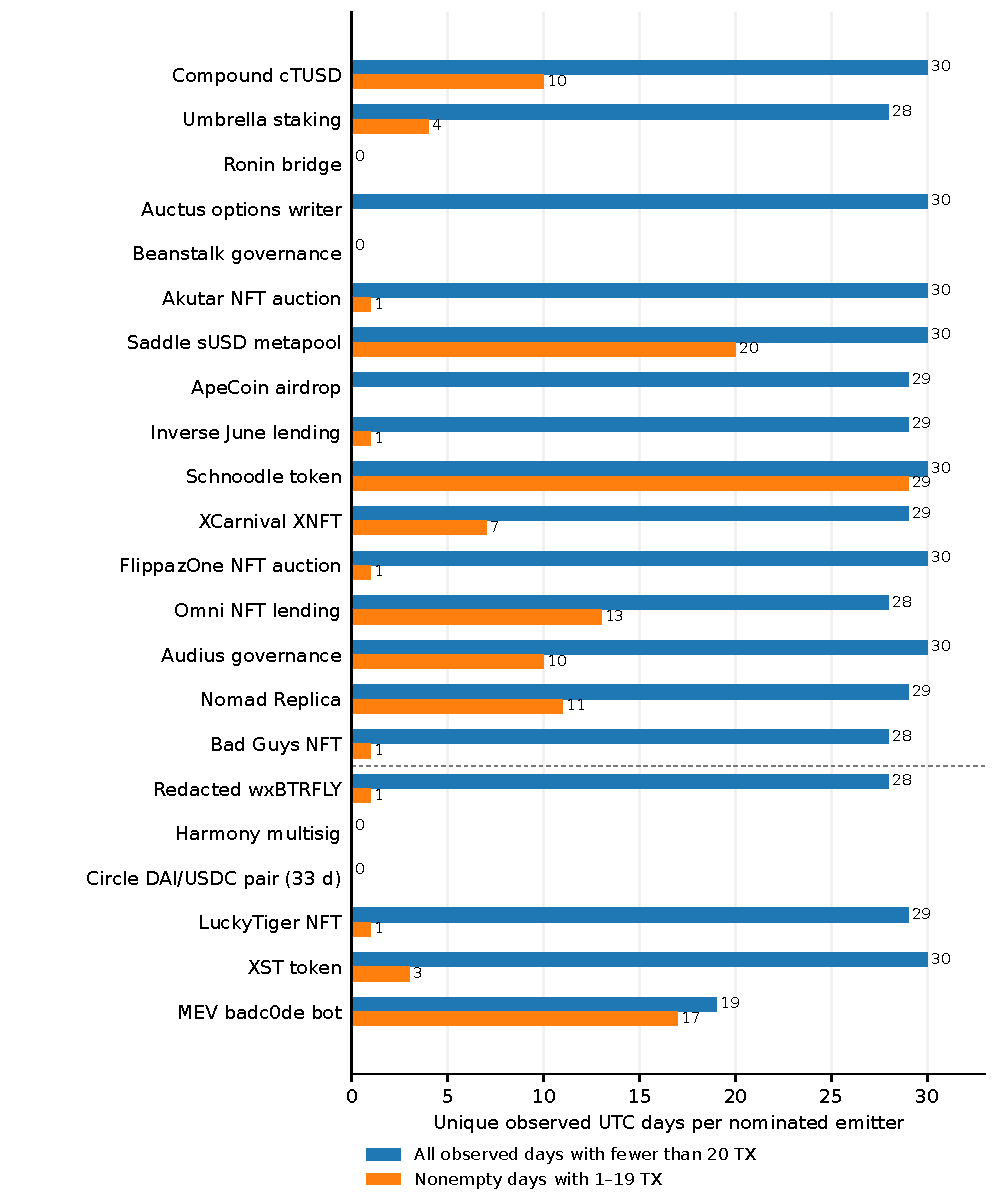
\includegraphics[width=\linewidth]{fig3_external_readiness_census.pdf}
\caption{Days below twenty selected transactions, among all observed dates and among nonempty dates, for each of 22 emitters. Circle uses the union of its two windows (33 dates); every other emitter has thirty. These are necessary feasibility bounds, not measured token ranks or exploit detections.}
\label{fig:newframe}
\end{figure}

\subsection{Seven exploratory fixed-emitter replays}\label{sec:sevenviews}
The follow-up subset was chosen after the four primary case outcomes and the original sixteen-emitter census were known. Low selected-transaction volumes were prioritized because complete source reconstruction was feasible within acquisition limits. The first wave comprised Umbrella, Inverse, Schnoodle and Omni; the second comprised Saddle, XCarnival and Audius. This favors sparse histories, so the fraction of rank-ineligible streams is not independent evidence of how common that failure is across DeFi. The fixed emitter boundaries were not changed after their score outcomes \citep{Umbrella2022Report,BlockSec2022Inverse,Schnoodle2022Analysis,SlowMist2023Omni,BlockSec2022Saddle,XCarnival2022Account,Audius2022Report}.

For every selected transaction, all original-Parquet row groups were checked to recover its identity, ordering and complete event count. Indexed payloads and success metadata were then matched to those original identities and counts. All 525 transactions were scored without incident references, preserving the rank/count rules and all history, policy and budget settings. A separate implementation reproduced 441/441 configurations, including eligibility, triggers, grouped candidates and exact emitted sequences. Reference joins followed scoring.

The reference column in Table~\ref{tab:sevenstreams} uses a uniform \emph{provisional candidate-identity} rule: a documented hash must be indexed as successful and selected by the fixed emitter within the observed window. It does not require that the hash's exploit role has been independently closed. Accordingly, the pending-role Umbrella candidate is included on the same identity basis as the other documented hashes; none of these denominators is an admitted-attack or incident-recall denominator. The table retains the original documentary candidate subset for comparability; the expanded role-specific audit below adds references without turning them into an attack denominator. Candidate stages outside the nominated emitter boundary are reported separately.

\begin{table}[htbp]
\centering\scriptsize
\caption{Seven exploratory emitter windows. Rank columns are daily / seven-day / captured-window history. Ready counts transactions with a history-eligible token rank; alerts use rank $1/20$, greedy $B=5$. The last column is count-rule exact matches / original selected documentary candidates, including unresolved roles. All primary rank-rule matches to these candidates are zero. Expanded role-specific references are reported separately; neither denominator measures attack recall.}
\label{tab:sevenstreams}
\setlength{\tabcolsep}{4pt}
\begin{tabularx}{\linewidth}{@{}>{\raggedright\arraybackslash}X r c c r l@{}}
\toprule
Fixed emitter view & Selected TX & Ready (d/7/30) & Rank alerts (d/7/30) & Count alerts & \shortstack{Count matches /\\selected original\\candidates} \\
\midrule
Umbrella & 92 & 0/0/0 & 0/0/0 & 0 & 0/1 (pending) \\
Saddle & 44 & 0/0/3 & 0/0/0 & 1 & 0/1 \\
Inverse & 71 & 20/20/20 & 3/3/3 & 2 & 0/1 \\
Schnoodle & 134 & 0/0/0 & 0/0/0 & 27 & \textbf{1/1 (count)} \\
XCarnival & 43 & 0/0/0 & 0/0/0 & 4 & 0/1 selected \\
Omni & 103 & 0/0/0 & 0/0/0 & 5 & 0/1 \\
Audius & 38 & 0/0/0 & 0/0/0 & 0 & 0/3 selected \\
\midrule
Total & 525 & --- & --- & --- & Nonindependent \\
\bottomrule
\end{tabularx}
\end{table}

No tested rank history is computable for Umbrella, Schnoodle, XCarnival, Omni or Audius. Saddle has three eligible cumulative-history transactions without a threshold crossing. Inverse has twenty eligible transactions and three rank notifications in every history mode, none matching its June 16 reference candidate. These results distinguish sparse token history from a defined but unexceptional score. They do not show that every low-volume stream must be ineligible: even thirty-eight selected transactions could, in principle, supply twenty qualifying same-token outflows.

Schnoodle's count rule emits 27 notifications on 134 selected transactions, or 20.15 per hundred transactions. One matches the reported June 18 execution \citep{Schnoodle2022Analysis}; the other 26 remain unadjudicated, limiting any selectivity claim. The reference at 07:05:24 UTC is that day's third count candidate, after 04:04:13 and 04:39:02. Greedy $B=1$ rejects it after exhausting the allocation (eighteen total notifications); $B=5$ delivers it (twenty-seven). At the same $B=5$, paced allocation also delivers it (twenty-four), whereas the token bucket with unit burst capacity suppresses it (twenty-one). A post-review sensitivity keeps the refill rate and daily cap fixed but increases burst capacity to five: with initial credit one, it delivers the reference among twenty-four notifications; initialized full, it reproduces all twenty-seven greedy notifications. Thus D can fail through either limited burst capacity or the hard daily cap.

The exact grouping boundary matters: Inverse includes candidates exactly 300 seconds apart, so $\Delta t\geq300$ s yields two count notifications rather than one. This is a deterministic boundary condition, not a tuned parameter.

\subsection{Role-specific observations in the three second-wave streams}\label{sec:threeroles}
A further audit examines all 125 selected transactions in Saddle, XCarnival and Audius, retaining every positive outflow's preceding transaction identities, history count and rank. It reproduces twelve primary rule/history cells and expands the documentary ledger to twelve role-specific hashes. These include preparation, failed governance attempts, extraction, rescue and asset sale; they cannot be pooled as twelve successful attacks. Table~\ref{tab:sevenstreams} retains the original reference subset, while the complete expanded observations are in the artifact.

The original V6.1 records retained derived features and payload digests but omitted raw indexed responses. Phase31 reacquires and retains full indexed responses for the unchanged 125-transaction population: 850 Saddle, 1,200 XCarnival and 53 Audius event rows. Offline re-extraction from a fresh archive reproduces every V6.1 canonical normalized event-payload digest, frozen feature and independently decoded token flow. Deliberate changes to response bytes, normalized events and success metadata are each rejected. This supplies reproducible indexed-source observations; it does not authenticate Ethereum receipt roots or close incident inventories.

\paragraph{Saddle: a strict maximum outside the score domain}
Of 44 selected transactions, 39 have a positive token outflow. BlockSec's report explicitly links the 07:40:24 UTC execution on 30 April \citep{BlockSec2022Saddle}. Its cumulative sUSD history contains sixteen prior positive values, three short of the required nineteen. The outflow is a strict observed maximum, but its descriptive rank $1/17$ still exceeds $1/20$ and lies outside the configured history domain. It is not a threshold crossing hidden solely by the history gate. The current count is nine core logs, below ten. A later transaction at 08:24:23 has the same reported attacker sender and a repeated pool sequence with proceeds returning to that sender. We classify it as a subsequent extraction by explicit chain-sequence inference, not as a closed incident inventory. Its cumulative sUSD history contains twenty prior values, passing B, but $q=3/21=1/7$ fails C. The two preceding values at least as large as the current outflow come from the first documented extraction and the intervening whitehat rescue: causal history is not necessarily benign history. The sole count notification occurs twelve seconds later, at 08:24:35: nine preceding logs plus one current log reach ten. It is not an exact match to the preceding extraction and its own role remains unadjudicated. The 08:04:55 whitehat rescue is separately linked by BlockSec's primary account \citep{BlockSec2023Rescue}; sharing an exploit mechanism does not make it a harmful extraction.

\paragraph{XCarnival: a different asset and observation boundary}
None of the 43 selected XNFT transactions has positive gross ERC-20-shaped core outflow. The frozen PoC and a separate investigator report identify two preparation/borrowing pairs \citep{DeFiHackLabs2026,SlowMist2022XCarnival}. Both preparation transactions are selected, whereas both borrowing transactions have zero XNFT-emitted logs in their retained indexed bundles. The documented economic extraction is native ETH borrowing through a different xToken proxy. Retaining more ERC-20 history at XNFT cannot repair this mismatch. One newly documented preparation reaches twenty-four core logs in the count window but is suppressed by grouping; this is distinct from budget rejection. The four emitted count notifications are not four established exploit detections.

\paragraph{Audius: governance outcome differs from transaction status}
The official post-mortem identifies an initial proposal attempt absent from the original four-hash PoC list \citep{Audius2022Report}. It is already present in the selected 38-transaction stream: the Ethereum transaction succeeds, but the governance proposal fails. The expanded ledger separates that attempt, renewed initialization/proposal, voting, treasury extraction and the later sale. Treasury extraction at 23:11:36 UTC on 23 July is the only positive AUDIO outflow in the entire captured governance stream. It has zero prior same-token positive values under all three histories and only three current-window core logs. The subsequent sale has no governance-emitter event and lies outside the fixed view. These observations attribute the nonnotifications to feature history and boundaries without treating setup, unsuccessful proposals and sale as interchangeable attacks.

\subsection{Nomad: an attack-day traffic burst and dispatch limits}\label{sec:nomad}
Nomad was selected after review for its 930-transaction census. Before scoring, we retained the original Replica address and 3 July--1 August 2022 window. Of these transactions, 884 occur on the attack day and only forty-six in the preceding twenty-nine days; this is not a sustained high-traffic history. Complete normalized original-AWS event bundles and transaction \texttt{receipt\_status} were retained. A standalone implementation verified all 930 transactions, 3,507 events and 63 fixed policy cells; acquisition interruptions are documented separately.

Of the selected transactions, 905 contain 1,157 positive ERC-20-shaped transfer events, but none supplies positive external outflow from the fixed Replica. This boundary failure is expected from the architecture: Replica processes and dispatches messages, while BridgeRouter releases escrow or mints assets \citep{NomadArchitecture,Nomad2022RCA}. Rank readiness is zero under every history.

After fixed scoring, a provisional hash join used the protocol team's published hack dataset at immutable commit \texttt{ba9adb9} \citep{Nomad2022HackData}. Its 960 hashes include 877 selected transactions in our stream; thirty-nine concern other Replicas and forty-four occur after our captured last block. All twelve count-rule grouped candidates belong to that public list. Greedy $B=5$ emits five and rejects seven under its hard daily cap. The first source-listed transaction is at 21:32:31 UTC, but the first count candidate is at 22:43:32. The fifth notification exhausts the cap at 23:17:33, and the first rejection follows at 23:23:01. Dispatch therefore suppresses protocol-listed candidates. List membership does not adjudicate malicious intent or establish a complete execution inventory; these joins do not estimate incident recall or precision. The boundary and rule remain fixed.

\section{Discussion: implications for reliable monitoring software}\label{sec:discussion}
\subsection{An explicit A--D validation contract}
The computation can be decomposed into four stages. \emph{A: observation}: the selected transaction supplies the measured feature, such as a positive core-boundary token outflow. \emph{B: computability}: the feature has its required prior state and valid domain; for the rank this means nineteen earlier positive values of the same token. \emph{C: triggering}: the defined score crosses its fixed threshold, here $q\leq1/20$. \emph{D: dispatch}: grouping and daily allocation admit a notification. These stages apply to a specified rule; the count comparator has a different B/C condition from the token rank.

Security-\emph{construct alignment} is a separate interpretation obligation: the observed feature must represent the hypothesized exploit mechanism before a notification can be interpreted as evidence of that mechanism. Mechanism relevance is not required to compute or emit a numerical alert. Table~\ref{tab:abc} separates observed outflow, prior samples and rank outcomes in the primary executions; the Schnoodle and Nomad count comparisons provide concrete D failures once candidates exist.

\begin{table}[htbp]
\centering\footnotesize
\caption{Primary rank conditions at known executions. The A column describes observed flow and any construct mismatch; relevance to the exploit is separate from numerical computability. Rari views share one execution. Primary Bacon/Rari rank candidates were not budget-blocked.}
\label{tab:abc}
\setlength{\tabcolsep}{3pt}
\begin{tabularx}{\linewidth}{p{2.0cm} >{\raggedright\arraybackslash}X >{\raggedright\arraybackslash}p{2.0cm} >{\raggedright\arraybackslash}X}
\toprule
View & A: observed boundary & B: previous samples & C: rank; exact hit \\
\midrule
Li.Fi & Core flow misses user approval drain & USDC: 55 & $54/56$; no \\
Revest & Token outflows present & RENA/ECO: 0 & Undefined; no \\
Bacon proxy & USDC core outflow & USDC: 32 & $1/33$; cumulative \\
Rari fETH & Positive core outflow & fETH: 23 (7d) & $1/24$; 7d, cumulative \\
Rari fUSDC & Positive ERC-20 outflow & USDC 26/63; fUSDC 22/33 & 7d: $1/27$, $1/23$; 30d: $1/64$, $1/34$; hit \\
Rari Comptroller & No positive ERC-20 core outflow & None & Undefined; count hit \\
\bottomrule
\end{tabularx}
\end{table}

The table's Li.Fi row illustrates the distinction: an observed USDC outflow and sufficient history allow a score, but the flow is not the user allowance drain and its rank is $54/56$. Revest lacks the required same-token history. Bacon and Rari yield exact matches under retained history, without proving that outflow magnitude recognizes reentrancy. Missing positive ERC-20 flow at the Comptroller does not imply absence of native-asset transfers elsewhere in the transaction.

\subsection{What the history intervention establishes}
The condition $N\geq20$ follows directly from the configured rank and is not itself a new scientific result. The empirical question is which observations count toward $N$ and whether they precede the evaluated transaction. Full-day volume, positive token-specific observations and strictly preceding history are different quantities. The Bacon/Rari timing results demonstrate that a sufficient end-of-day count can coexist with attack-time ineligibility.

Longer history is not evaluated solely by the number of newly defined scores: it also changes their relative ranks. Li.Fi and Revest gain eligible transactions without new known-execution matches, while Bacon and Rari gain exact matches. These are counterfactual historical replays with fixed rules, not randomized or prospective deployment outcomes. The three Rari views still represent one execution.

\subsection{Scope of the extension evidence}\label{sec:transport}
The comparison-contract census demonstrates feature-domain differences on the \emph{same} discrete observations: a five-sample EWMA is almost always defined, whereas a nineteen-sample positive-MAD statistic is often undefined. This comparison does not estimate the ERC-20 rank's availability. Likewise, the completed source census supplies a traffic upper bound, not token-specific readiness.

The seven low-volume replays distinguish ineligibility from defined scores and notifications, but their five ineligible views cannot estimate prevalence. Nomad adds an attack-day burst: its Replica boundary predictably lacks token outflow, while its count rule supplies protocol-listed candidates rejected by the daily cap. This separates an architecture-dependent A failure from a realized D rejection without removing purposive sampling or reference-role limitations.

Count and rank rules match different documented transactions in these traces: count matches Li.Fi and Schnoodle, whereas the Bacon match requires retained token history. This is not evidence that an ensemble improves general detection. Schnoodle's 20.15 notifications per hundred selected transactions, $B=1$ rejection and policy-dependent $B=5$ outcome show why notification burden and dispatch must accompany an exact-match claim. Unknown notifications are neither confirmed false positives nor evidence of early warning.

\subsection{Implications for monitor evaluation}
An evaluation should specify the relevant security transition and observable contracts, verify source completeness, report undefined features separately from defined low scores, measure state strictly before the reference execution, and retain both candidate and dispatch decisions. Reference joining should follow fixed scoring. Reproducing a rank formula is insufficient if observation boundaries, state initialization or notification delivery are omitted from the acceptance criteria. These checks improve interpretability; they do not establish a detector's population accuracy or ability to prevent an atomic transaction.

\section{Threats to validity}\label{sec:validity}
\paragraph{Selection and independence} The primary four-family cohort was incident-informed; Bacon/Rari followed exposure to Li.Fi/Revest. The completed source frame covers the frozen catalogue's Ethereum files, but its period, catalogue coverage and interpreted component boundaries do not represent all DeFi incidents. The seven replay views were chosen partly for low traffic after the original sixteen-window census. The Nomad attack-day burst was also purposively selected after review. These readiness frequencies cannot validate cross-protocol transportability. The comparison contracts are nonrandom and unmatched on role or deployment date. Dependent UTC days, multiple Rari views and deterministic configuration cells must not be treated as independent incidents. No population significance or superiority claim follows.

\paragraph{Reference roles and notification interpretation} Primary execution inventories are known subsets, especially for Rari's multiple pools. Exploratory joins use documented candidate identities, including unresolved roles; they are not interchangeable with admitted successful executions. Nomad uses a later protocol-published hash list whose entries are not independently adjudicated as malicious executions. Missing matches cannot quantify incident-wide recall, and unadjudicated notifications cannot establish precision, false-positive rate or missed economic loss.

\paragraph{Sources and feature boundaries} Original Parquet identities and event counts were cross-checked against indexed bundles. Complete original payload agreement was checked for the ten decisive Bacon/Rari transactions, but not for all 667 selected transactions or against receipt roots. Phase31 closes the earlier raw-payload retention gap for all 125 second-wave transactions: retained indexed responses reproduce their 2,103 event rows and every frozen feature. This additional check does not cover all earlier Bacon/Rari or first-wave transactions, and remains indexer evidence rather than receipt-root authentication. Nomad instead retains normalized original-AWS event bundles and dataset transaction status, but not the original Parquet bodies needed for offline byte-to-normalization reconstruction. Source statuses, incomplete incident narratives, nominated addresses and syntactic event parsing remain limitations. Native ETH, internal calls, nonstandard token behavior and state invariants can fall outside the measured feature. A silent emitter is not proof of an inactive or undeployed contract.

\paragraph{Time and operations} Retained histories start cold within a thirty-day capture; grouping and budget state reset at UTC midnight. Fork-date windows are not exact attack-time windows, and their final date can include post-fork activity. Block timestamps are historical event times, not measured data-delivery or alert latency. An alert on an atomic exploit transaction does not demonstrate prevention or reduced loss.

\paragraph{Implementation checks} Independent implementations reproduce the recorded decisions but cannot certify every source narrative or full historical completeness. Sensitivity cells do not constitute optimized new detector parameters. Notification counts measure emitted workload, not analyst time or operational utility. Final software and bibliography checks constrain reporting errors without removing these sampling and construct limitations.

\section{Conclusion}\label{sec:conclusion}
Across four Ethereum incident families and five admitted executions, the daily-reset token-outflow rank produced no exact known-execution notifications. Longer causal histories yielded matches for Bacon and Rari but not Li.Fi or Revest. End-of-day volume concealed attack-time history deficits, and exact notification did not establish exploit-mechanism recognition.

The extensions distinguish traffic feasibility from feature computability. Across 22 census emitters, 130 of 277 nonempty days failed the twenty-transaction gate; 386 additional days were silent. On the comparison-contract event counts, z-score, positive-MAD and EWMA readiness differed substantially. Seven low-volume replays added verified token-level outcomes but cannot establish prevalence. Nomad's traffic is concentrated on the attack day; its Replica boundary predictably supplies no positive core outflow, whereas the count-rule daily cap rejects seven protocol-listed candidates. Schnoodle's count match occurred in a stream notifying 20.15\% of selected transactions. It disappeared under a one-alert budget and under token-bucket allocation with unit burst capacity at the original five-alert cap.

The supported evaluation requirement is to report observation, causal feature domain, threshold crossing and delivered notification separately, then assess security-construct alignment. Broader protocol coverage and closed execution roles are needed for cross-protocol performance claims.

\section*{Data, code and reproducibility}
The revision and Phase31--32 evidence are identified by the release reference \href{https://github.com/KuznetsovKarazin/blockchain-analytics-lab/tree/article2-jss-v8-2026-10-30}{\texttt{article2-jss-v8-2026-10-30}} \citep{Kuznetsov2026Artifacts}. The immutable V6.1 baseline remains \texttt{article2-jss-v6.1-2026-10-29}, commit \texttt{651daa926bb3803ad76227389a4fb35c1027da63}; the sealed primary baseline is \texttt{e720697bc3986dd291a7047c580cf973ae6e5567}. The V6 research line branched from Phase27 commit \texttt{78baeb5} rather than continuing the V5 manuscript revision. V7 remains published at commit \texttt{aab963c5c5aa60adb7af5f04bc86601f92c67b87}; original releases are unchanged. The accompanying README and manifests specify source pins, checksums and offline commands; no Zenodo DOI has been assigned.

Phase16--30 preserve the earlier source tiers. Phase31 retains full indexed responses for all 125 Saddle/XCarnival/Audius transactions and normalized original-dataset bundles for 930 Nomad transactions. Offline checks reproduce the three-case cohort's 2,103 event rows, canonical payload digests and frozen features, plus all 63 Nomad policy cells. Original Parquet byte-to-normalization extraction requires network access. Phase32 adds the completed catalogue census, protocol-list join, Saddle source check and burst-capacity sensitivity. The source-retention limits are specified in Section~\ref{sec:validity}; neither archive authenticates Ethereum receipt roots or closes incident inventories.

\section*{Competing interests}
The author reports financial support for this work from the European Union through PETs4DeFi (Grant Agreement No.~101308999).
\section*{Funding}
This work was supported by the European Union's Horizon Europe programme under Grant Agreement No.~101308999 (PETs4DeFi), supported by the European Cybersecurity Competence Centre. Views and opinions expressed are however those of the author only and do not necessarily reflect those of the European Union or the European Cybersecurity Competence Centre. Neither the European Union nor the European Cybersecurity Competence Centre can be held responsible for them.
\section*{Declaration of generative AI and AI-assisted technologies in the manuscript preparation process}
OpenAI ChatGPT and Codex assisted literature organization and manuscript preparation. AI-assisted content was checked against sources and reproducible calculations; the author takes responsibility for the final article.

\appendix
\renewcommand{\theHtable}{appendix.\Alph{section}.\arabic{table}}
\section{Complete primary notification ledger}\label{app:alerts}
\setcounter{table}{0}
Each row is one emitted rank-$1/20$, greedy $B=5$ notification. Token names are indicative; the CSV retains full contract addresses, ranks and transaction hashes. \textbf{Known} denotes an exact admitted execution; \textbf{Unknown} denotes an unadjudicated notification, not a false positive.
\begingroup\scriptsize\setlength{\tabcolsep}{3pt}
\begin{longtable}{p{1.85cm}p{1.0cm}p{2.3cm}p{3.0cm}p{1.2cm}}
\caption{Exact emitted-transaction ledger for the primary rank rule (greedy, $B=5$). Multiple entries at the same transaction represent alternative component-view simulations, not separate attacks.}\label{tab:alerts}\\
\toprule
View & History & UTC date and time & Triggering token(s) and rank(s) & Status \\
\midrule
\endfirsthead
\toprule
View & History & UTC date and time & Triggering token(s) and rank(s) & Status \\
\midrule
\endhead
Bacon & 30d & 2022-03-05 12:46 & USDC 1/33 & Known \\
Li.Fi & 30d & 2022-03-01 09:25 & USDC 1/20 & Unknown \\
Li.Fi & 30d & 2022-03-03 03:42 & USDC 1/22 & Unknown \\
Rari fUSDC & 30d & 2022-04-28 13:38 & USDC 1/53 & Unknown \\
Rari fUSDC & 30d & 2022-04-28 13:57 & USDC 1/27 & Unknown \\
Rari fUSDC & 30d & 2022-04-28 22:50 & USDC 1/58 & Unknown \\
Rari fETH & 30d & 2022-04-28 23:55 & fETH 1/30 & Unknown \\
Rari fUSDC & 30d & 2022-04-30 03:08 & fUSDC 1/24 & Unknown \\
Rari fETH & 30d & 2022-04-30 03:15 & fETH 1/37 & Unknown \\
Rari fUSDC & 30d & 2022-04-30 03:32 & fUSDC 1/25 & Unknown \\
Rari fETH & 30d & 2022-04-30 09:32 & fETH 1/42 & Known \\
Rari fUSDC & 30d & 2022-04-30 09:32 & USDC 1/64; fUSDC 1/34 & Known \\
Rari fUSDC & 30d & 2022-04-30 18:14 & USDC 1/37 & Unknown \\
Rari fUSDC & 7d & 2022-04-28 22:50 & USDC 1/22 & Unknown \\
Rari fETH & 7d & 2022-04-30 09:32 & fETH 1/24 & Known \\
Rari fUSDC & 7d & 2022-04-30 09:32 & USDC 1/27; fUSDC 1/23 & Known \\
Revest & 30d & 2022-03-24 23:57 & token 0x120a 2/64 & Unknown \\
Revest & 7d & 2022-03-23 01:04 & token 0x120a 1/20 & Unknown \\
Revest & 7d & 2022-03-24 23:57 & token 0x120a 1/57 & Unknown \\
\bottomrule
\end{longtable}
\endgroup


\section{Completed source census and initial reference preflight}\label{app:sourcecensus}
\setcounter{table}{0}
\small
\setlength{\LTcapwidth}{\linewidth}
\begin{longtable}{@{}p{6.9cm}rrrr@{}}
\caption{Source-transaction counts for 23 thirty-day emitter/fork windows across 22 emitters. Circle overlaps by 27 dates; the final row deduplicates dates. The two XST files share one window. These counts do not measure detections.}\label{tab:allcensus}\\
\toprule
Candidate emitter/window & TX & 0 TX/d & 1--19/d & $\geq20$/d\\
\midrule
\endfirsthead
\toprule
Candidate emitter/window & TX & 0 TX/d & 1--19/d & $\geq20$/d\\
\midrule
\endhead
Compound cTUSD sweepToken & 15 & 20 & 10 & 0\\
Umbrella Network staking & 92 & 24 & 4 & 2\\
Ronin Bridge Ethereum withdrawal & 18,522 & 0 & 0 & 30\\
Auctus options writer & 0 & 30 & 0 & 0\\
Beanstalk governance & 12,392 & 0 & 0 & 30\\
Akutar NFT auction & 1 & 29 & 1 & 0\\
Saddle sUSD metapool & 44 & 10 & 20 & 0\\
ApeCoin airdrop claim & 10,938 & 29 & 0 & 1\\
Inverse Finance June lending & 71 & 28 & 1 & 1\\
Schnoodle ERC777 token & 134 & 1 & 29 & 0\\
XCarnival XNFT & 43 & 22 & 7 & 1\\
FlippazOne NFT auction & 1 & 29 & 1 & 0\\
Omni NFT lending & 103 & 15 & 13 & 2\\
Audius governance & 38 & 20 & 10 & 0\\
Nomad Bridge replica & 930 & 18 & 11 & 1\\
Bad Guys by RPF NFT & 1,456 & 27 & 1 & 2\\
\midrule
Original sixteen & 44,780 & 302 & 108 & 70\\
\midrule
RedactedCartel wxBTRFLY & 167 & 27 & 1 & 2\\
Harmony Ethereum multisig & 1,554 & 0 & 0 & 30\\
Circle pair, fork 15,331,019 & 3,237 & 0 & 0 & 30\\
Circle pair, fork 15,354,437 & 3,254 & 0 & 0 & 30\\
LuckyTiger NFT & 220 & 28 & 1 & 1\\
XST token & 4 & 27 & 3 & 0\\
MEVbadc0de contract & 1,276 & 2 & 17 & 11\\
\midrule
All 23 windows (multiplicity) & 54,492 & 386 & 130 & 174\\
All 22 emitters (unique dates) & 51,452 & 386 & 130 & 147\\
\bottomrule
\end{longtable}
\normalsize

\begin{table}[H]
\centering\small
\caption{Initial reference preflight for twelve original nominations. \emph{Core present} denotes emitter matching, not notification. All transactions succeeded; roles were not adjudicated. Unknown pagination was later resolved where complete bundles were reconstructed.}
\label{tab:refpreflight}
\begin{tabularx}{\linewidth}{@{}>{\raggedright\arraybackslash}X r r r@{}}
\toprule
Case & \shortstack{Indexed\\TX} & \shortstack{Core\\present} & \shortstack{Within PoC\\window}\\
\midrule
Umbrella Network staking & 1 & 1/1 & 1/1\\
Beanstalk governance & 1 & 1/1 & 0/1\\
Akutar NFT auction & 1 & 0/1 & 0/1\\
Saddle sUSD metapool & 1 & 1/1 & 1/1\\
ApeCoin airdrop claim & 1 & 1/1 & 1/1\\
Inverse Finance June lending & 1 & 1/1 & 1/1\\
Schnoodle ERC777 token & 1 & 1/1 & 1/1\\
XCarnival XNFT & 2 & 1/2 & 2/2\\
Omni NFT lending & 1 & 0/1 (1 unknown) & 1/1\\
Audius governance & 4 & 3/4 & 4/4\\
Nomad Bridge replica & 2 & 1/2 & 2/2\\
Bad Guys by RPF NFT & 1 & 1/1 & 1/1\\
\midrule
All candidate references & 17 & 12/17 (1 unknown) & 15/17\\
\bottomrule
\end{tabularx}
\end{table}


\bibliographystyle{elsarticle-harv}
\begingroup\footnotesize\setlength{\bibsep}{2pt}\sloppy\bibliography{references}\endgroup
\end{document}
